\documentclass[titlepage]{article}

\usepackage[margin=1in]{geometry}
\usepackage{csquotes}
\usepackage{fancyhdr}
\usepackage{marginnote}
\usepackage{enumitem}
\usepackage{siunitx}
\usepackage[style=chem-acs]{biblatex}
\usepackage{pdfpages}
\usepackage{amsmath,amssymb}
\usepackage{subcaption}
\usepackage{mhchem}
\usepackage{chemfig}
\usepackage[hidelinks]{hyperref}

\MakeOuterQuote{"}

\fancypagestyle{main}{
    \fancyhf{}
    \fancyhead[L]{\leftmark}
    \fancyhead[R]{CHEM 22000}
    \fancyfoot[R]{Labalme\ \thepage}
}
\fancypagestyle{plain}{
    \fancyhf{}
    \renewcommand{\headrulewidth}{0pt}
}

\reversemarginpar

\setlist[itemize,3]{label={\scriptsize$\blacksquare$}}

\DefineBibliographyStrings{english}{bibliography={References}}

\setchemfig{atom sep=2em,fixed length=true,bond offset=3pt,cram width=3pt}
\setcharge{extra sep=3pt}

\newcommand{\R}{\mathbb{R}}
\newcommand{\e}[1][]{\text{e}^{#1}}

\usepackage{subfiles}

\addbibresource{../../main.bib}

\title{Separation and Analysis of Three Unknown Solids}
\author{
    Steven Labalme\\
    \normalsize Lab Section 1A05
}

\begin{document}




\maketitle



\pagestyle{main}
\renewcommand{\leftmark}{Lab Assignment 1d}
\setitemize{label={--}}
\section*{Figure}
\begin{figure}[h!]
    \centering
    \footnotesize
    \hspace*{-4mm}
    \begin{tikzpicture}[
        entity/.style={draw,inner sep=4pt},
        every path/.style={semithick}
    ]
        \node (1) [entity] {Unknown mixture of solids};
        \node (2) [entity,below=of 1] {3 unknowns present}
            edge [stealth-] node[right]{TLC (1:1 hexanes to ethyl acetate)} (1)
        ;
        \node (3b) [below=of 2] {}
            (3b.center) edge node[right,align=left]{Dissolve in \ce{CH2Cl2}\\Gravity filtration} (2)
        ;

        \node (3a) [left=6cm of 3b] {}
            (3a.center) edge (3b.center)
        ;
        \node (4a) [entity,below=of 3a] {Unknown A}
            edge [stealth-] (3a.center)
        ;
        \node (5a) [entity,below=of 4a,align=center] {
            Resorcinol\\[5pt]
            Benzene-1,3-diol\\[5pt]
            \chemfig{*6(=-=(-OH)-=(-HO)-)}\\[5pt]
            MP range: $\Delta\SI{0.9}{\celsius}$ --- good purity
        }
            edge [stealth-] node[right]{Melting point} (4a)
        ;

        \node (3c) [right=3cm of 3b] {}
            (3c.center) edge (3b.center)
        ;
        \node (4b) [entity,below=of 3c] {Unknowns B \& C}
            edge [stealth-] (3c.center)
        ;
        \node (5c) [below=4mm of 4b] {}
            (5c.center) edge node[right]{Extraction (\ce{NaHCO3})} (4b)
        ;

        \node (5b) [left=3cm of 5c] {}
            (5b.center) edge (5c.center)
        ;
        \node (8a) [entity,below=2cm of 5b] {Basic layer (Unknown B)}
            edge [stealth-] (5b.center)
        ;
        \node (9a) [entity,below=of 8a] {Unknown B precipitate}
            edge [stealth-] node[right]{\ce{HCl}} (8a)
        ;
        \node (10a) [entity,below=of 9a] {Unknown B}
            edge [stealth-] node[right]{Vacuum filtration} (9a)
        ;
        \node (11a) [entity,below=of 10a,align=left] {
            One of the following:\\
            1. \emph{p}-Anisic acid\\
            2. Aspirin\\
            3. Benzoic acid\\
            4. \emph{trans}-Cinnamic acid\\
            5. Gallic acid\\
            6. Isophthalic acid\\
            7. Oxalic acid
        }
            edge [stealth-] node[right]{IR spectroscopy} (10a)
        ;
        \node (12a) [entity,below=of 11a,align=center] {
            \emph{trans}-Cinnamic acid\\[5pt]
            (2E)-3-phenylprop-2-enoic acid\\[5pt]
            \chemfig{*6(=-=(-=_[:-30]-[:30](=[2]O)-[:-30]OH)-=-)}\\[5pt]
            TLC dots match exactly --- great purity
        }
            edge [stealth-] node[right]{TLC} (11a)
        ;

        \node (5d) [right=3cm of 5c] {}
            (5d.center) edge (5c.center)
        ;
        \node (6) [entity,below=4mm of 5d] {Organic layer (Unknown C)}
            edge [stealth-] (5d.center)
        ;
        \node (7) [below=4mm of 6] {}
            (7.center) edge node[right]{Extraction (\ce{NaHCO3})} (6)
            (7.center) edge ++(-6,0)
        ;
        \draw [-stealth] (7.center) ++(-6,0) -- ++(0,-0.5);
        \node (8b) [entity,below=4mm of 7] {Organic layer (Unknown C)}
            edge [stealth-] (7.center)
        ;
        \node (9b) [entity,below=of 8b] {Dissolved Unknown C}
            edge [stealth-] node[right]{Dry (\ce{Na2SO4})} (8b)
        ;
        \node (10b) [entity,below=of 9b] {Unknown C}
            edge [stealth-] node[right]{Rotavap} (9b)
        ;
        \node (11b) [entity,below=of 10b] {Unknown C}
            edge [stealth-] node[right,align=left]{Dissolve in \ce{EtOH}\\Activated charcoal\\Recrystallization} (10b)
        ;
        \node (12b) [entity,below=of 11b,align=center] {
            \emph{trans}-Stilbene\\[5pt]
            1,1'-[(E)-ethene-1,2-diyl]dibenzene\\[5pt]
            \chemfig{*6(=-=(-=_[:-30]-[:30]*6(=-=-=-))-=-)}\\[5pt]
            Identical IR spectra fingerprints --- great purity
        }
            edge [stealth-] node[right]{IR spectroscopy} (11b)
        ;
    \end{tikzpicture}
    \caption{Isolation and purification process for a selection of unknown solids.}
    \label{fig:figure}
\end{figure}



\section*{Lab Report}
\begin{enumerate}
    \item What is the identity of unknown A and how did you determine this?
    \begin{itemize}
        \item Unknown A is resorcinol. The experimental melting point range of $\SIrange{108.7}{109.6}{\celsius}$ falls within the known melting point range of resorcinol, and is disjoint from all other known melting point ranges.
    \end{itemize}
    \item Comment on the relative purity of unknown A and how you determined this.
    \begin{itemize}
        \item Unknown A is pretty pure. With a ramp rate of $\SI[per-mode=symbol]{1}{\celsius\per\minute}$, the change in temperature from when the sample started to melt to when it finished melting was only $\SI{0.9}{\celsius}$.
    \end{itemize}
    \item What is the identity of unknown B and how did you determine this? Discuss both the IR and TLC data. Include a published IR spectrum in your report and comment on similarities between it and the spectrum you obtained.
    \begin{figure}[h!]
        \centering
        \begin{subfigure}[b]{0.49\linewidth}
            \centering
            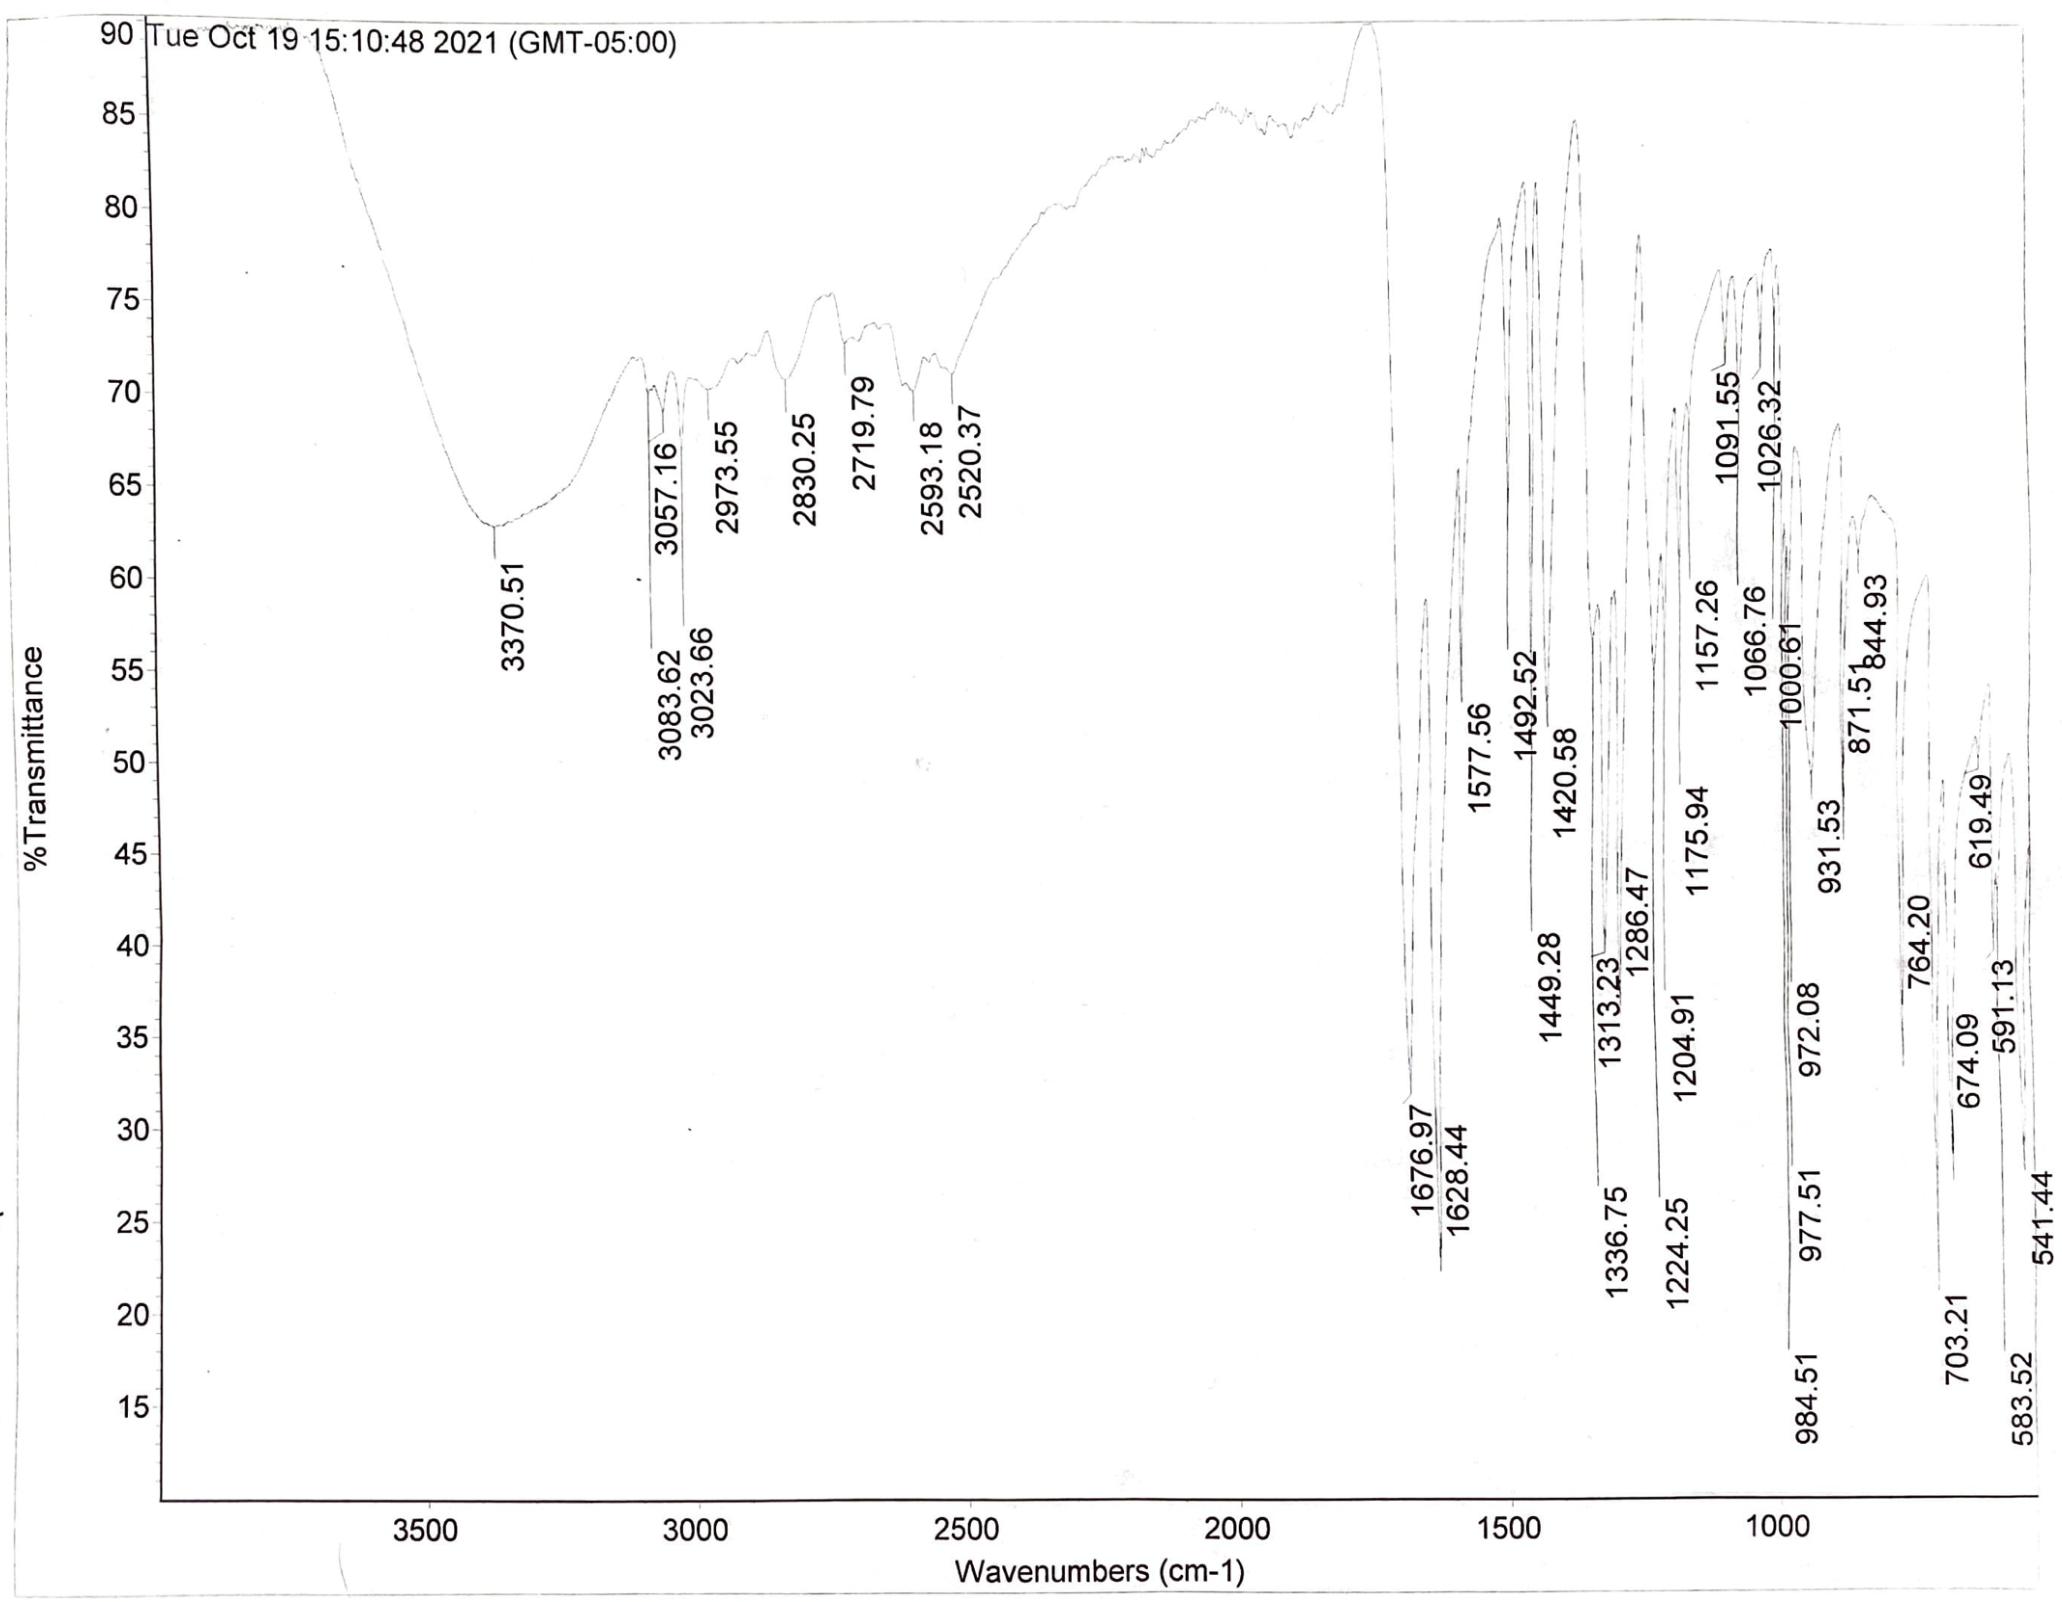
\includegraphics[width=0.9\linewidth]{../../ExtFiles/transCinnamicAcid-IRSpectrum-Experimental.png}
            \caption{Experimental.}
            \label{fig:IR-Ba}
        \end{subfigure}
        \begin{subfigure}[b]{0.49\linewidth}
            \centering
            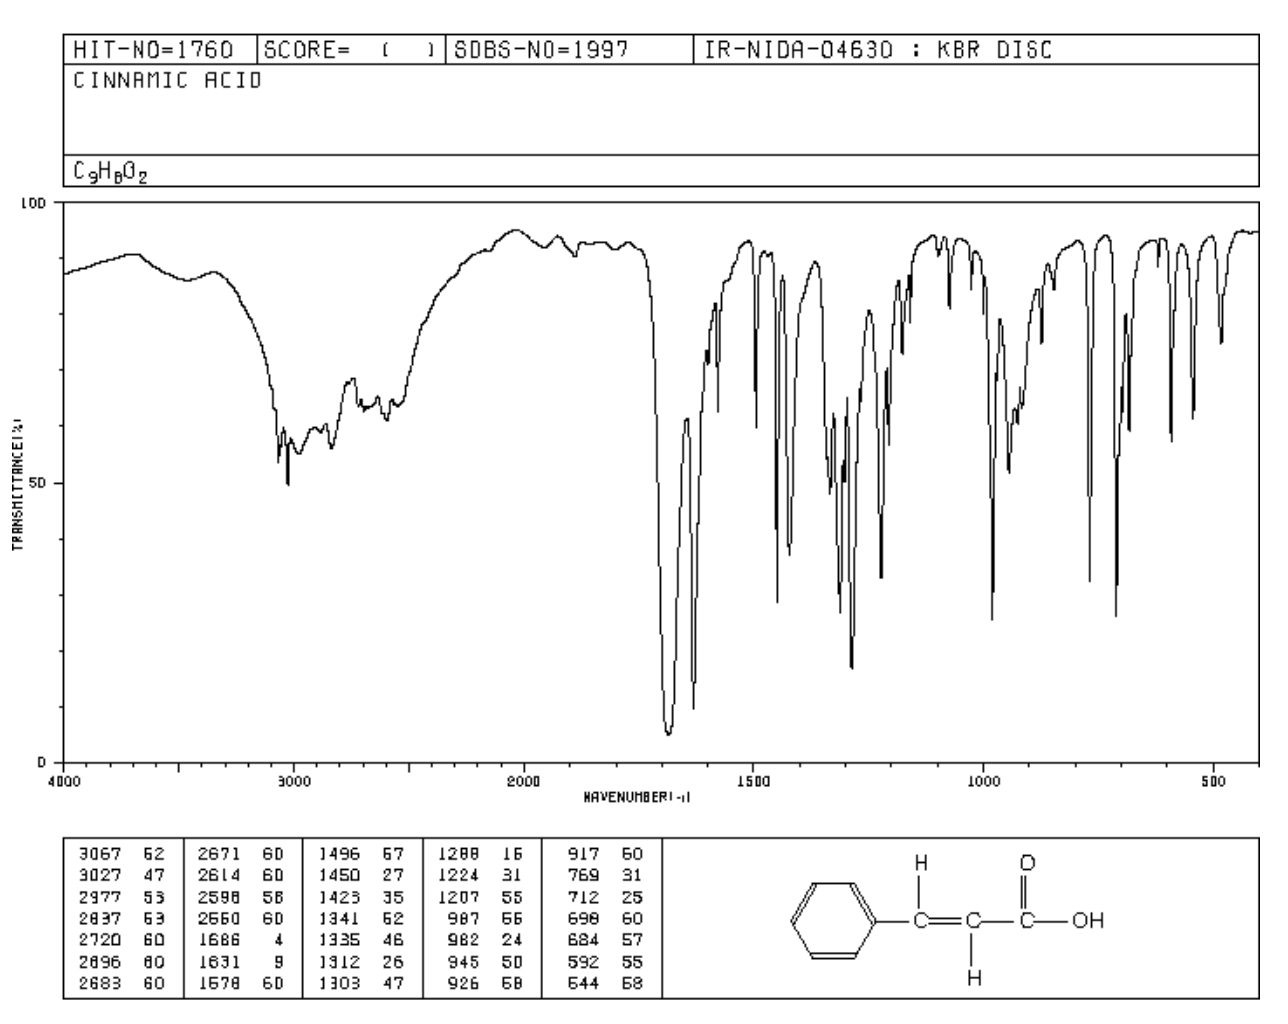
\includegraphics[width=0.9\linewidth]{../../ExtFiles/transCinnamicAcid-IRSpectrum-Known.png}
            \caption{Known\supercite{bib:transCinnamicAcid-IRSpectrum}.}
            \label{fig:IR-Bb}
        \end{subfigure}
        \caption{\emph{trans}-cinnamic acid IR spectra.}
        \label{fig:IR-B}
    \end{figure}
    \begin{itemize}
        \item Unknown B is \emph{trans}-cinnamic acid. The experimentally obtained IR spectrum contains a distinct carboxylic acid peak (see Figure \ref{fig:IR-Ba}), leading to the conclusion that B must be one of the seven possible compounds containing carboxylic acid functional groups. Comparison of these seven compounds with unknown B on the same TLC plates yielded identical and indistinguishable motion for unknown B and \emph{trans}-cinnamic acid. Lastly, Figure \ref{fig:IR-B} shows that the IR spectrum of unknown B and that of \emph{trans}-cinnamic acid match nicely, especially in the fingerprint region.
    \end{itemize}
    \item Was the identity of unknown B definitive? In other words, were there any other possibilities?
    \begin{itemize}
        \item Yes, it was definitive. Based on the exact match of the TLC dots (see notebook pages for sketch), unknown B is certainly \emph{trans}-cinnamic acid.
    \end{itemize}
    \item What is the identity of unknown C and how did you determine this?
    \begin{itemize}
        \item Unknown C is \emph{trans}-stilbene. The IR spectrum obtained for the compound has a fingerprint region that matches nearly perfectly with the fingerprint region of the known IR spectrum of \emph{trans}-stilbene.
    \end{itemize}
    \item Comment on the relative purity of unknown C and how you determined this.
    \begin{itemize}
        \item Unknown C is quite pure. As per the above, the experimental and known IR spectra match nearly exactly.
    \end{itemize}
\end{enumerate}
\newpage



\printbibliography




\end{document}